\documentclass[tikz,border=6pt]{standalone}
\usepackage{amsmath,amssymb}
\usetikzlibrary{angles,quotes,calc}
\begin{document}
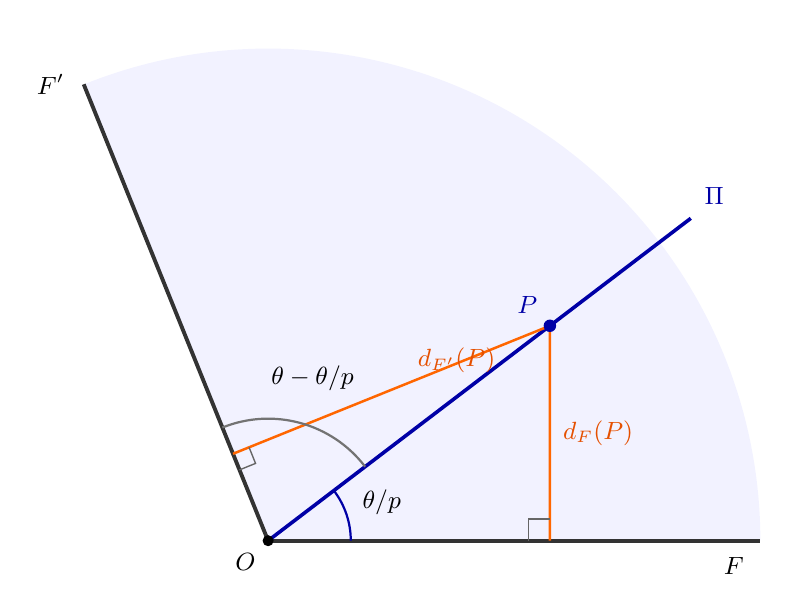
\begin{tikzpicture}[scale=1.25,
  face/.style={line width=1.4pt,draw=black!80},
  sect/.style={line width=1.3pt,draw=blue!65!black},
  perp/.style={line width=0.9pt,draw=orange!80!red},
  lbl/.style={font=\small}]
\def\th{112}
\def\ph{37.333}
\coordinate (O) at (0,0);
\coordinate (F) at (5,0);
\coordinate (G) at (\th:5);
\coordinate (S) at (\ph:5.4);
\coordinate (P) at (\ph:3.6);
\coordinate (PF) at ($(O)!(P)!(F)$);
\coordinate (PG) at ($(O)!(P)!(G)$);
\fill[blue!5] (O) -- (F) arc[start angle=0,end angle=\th,radius=5] -- cycle;
\draw[face] (O) -- (F) node[lbl,below left=2pt] {$F$};
\draw[face] (O) -- (G) node[lbl,left=3pt] {$F'$};
\draw[sect] (O) -- (S) node[lbl,above right=1pt,text=blue!65!black] {$\Pi$};
\draw[perp] (P) -- (PF) node[pos=0.5,lbl,right=1pt,text=orange!70!red!90!black] {$d_F(P)$};
\draw[perp] (P) -- (PG) node[pos=0.45,lbl,above right=0pt,text=orange!70!red!90!black] {$d_{F'}(P)$};
\draw[black!60,line width=0.5pt] ($(PF)+(0,0.22)$) -- ++(-0.22,0) -- ++(0,-0.22);
\pic[draw=black!60,line width=0.5pt,angle radius=0.22cm] {right angle=O--PG--P};
\pic[draw=blue!65!black,line width=0.8pt,angle radius=1.05cm,"$\theta/p$",angle eccentricity=1.45,font=\small] {angle=F--O--S};
\pic[draw=black!55,line width=0.8pt,angle radius=1.55cm,"$\theta-\theta/p$",angle eccentricity=1.38,font=\small] {angle=S--O--G};
\fill[black] (O) circle (1.6pt) node[lbl,below left=1pt] {$O$};
\fill[blue!65!black] (P) circle (1.8pt) node[lbl,above left=1pt] {$P$};
\end{tikzpicture}
\end{document}
